\documentclass{report}
\usepackage[latin1]{inputenc}
\usepackage{hyperref}
\usepackage{graphicx}

\title{%
    \begin{minipage}\linewidth
        \centering
        Rapport de projet\\
        \large WEB API REST - Gestion d'une mediath\`{e}que
    \end{minipage}
}

\author{
	\textbf{Marie-Laure FASQUEL} \\
	\'{E}tudiante M1 ISIDis - Universit\'{e} du Littoral C\^{o}te d'Opale\\
	fasquel.ml@gmail.com\\
	\\
	\textbf{K\'{e}vin VASSEUR} \\
	\'{E}tudiant M1 ISIDis - Universit\'{e} du Littoral C\^{o}te d'Opale\\
	vasseur.isn@gmail.com\\
}
\date{\textbf{\today}}


\begin{document}
	\maketitle
	\begin{abstract}
		Le but de ce projet est de cr\'{e}er une WEB API REST qui g\`{e}re une mediath\`{e}que. La date de lancement de ce projet est dat\'{e} au 13 mars 2017 et sa date de livraison est fix\'{e}e au samedi 1 avril 2017. Nous avons libre choix dans les technologies employ\'{e}es. \\
	\end{abstract}
	
	\tableofcontents	
	
	\chapter{Pr\'{e}sentation}
	% ########## TECHNOS ##########
	
	
	\section{Technologies}
		\subsection{Technologies utilis\'{e}es}
			\subsubsection{Environnement WAMP}
			\textbf{Version :} 3.0.6 \\
			\begin{itemize}
			\item PHP : 5.6.25
			\item MySQL : 5.7.14
			\item Apache : 2.4.23
			\end{itemize}
			
			\subsubsection{Cake PHP}
			\textbf{Version :} 2.9.? (au lieu de la 3.4.3) \\
			
			\subsubsection{Bootstrap}
			\textbf{Version :} 3 \\		
			
		\subsection{Niveau des membres}
			\subsubsection{Marie-Laure FASQUEL}
			...
			\subsubsection{K\'{e}vin VASSEUR}
			...
			
	% ########## CONSIGNES ##########		
	\section{Consignes}
	\begin{enumerate}
		\item \textbf{/books} - \textit{donne la liste des livres (m\'{e}thode Get)}
		\item \textbf{/books} - \textit{cr\'{e}e un livre dans la base (m\'{e}thode Post)}
		\item \textbf{/books/[int]} - \textit{donne le livre \`{a} l'identifiant donn\'{e} (m\'{e}thode Get)} 
		\item \textbf{/books/[int]} - \textit{supprime un livre dans la base (m\'{e}thode Delete)} 
		\item \textbf{/books/[int]} - \textit{met \`{a} jour un livre dans la base (m\'{e}thode Put}) 
		\item \textbf{/members/[int]/books} - \textit{affiche les livres pour le membre donn\'{e} (m\'{e}thode Get)} 
	\end{enumerate}
	
	
	\section{R\'{e}sultats en utilisant PostMan}
		\subsection{Question 1}
		\begin{center}
			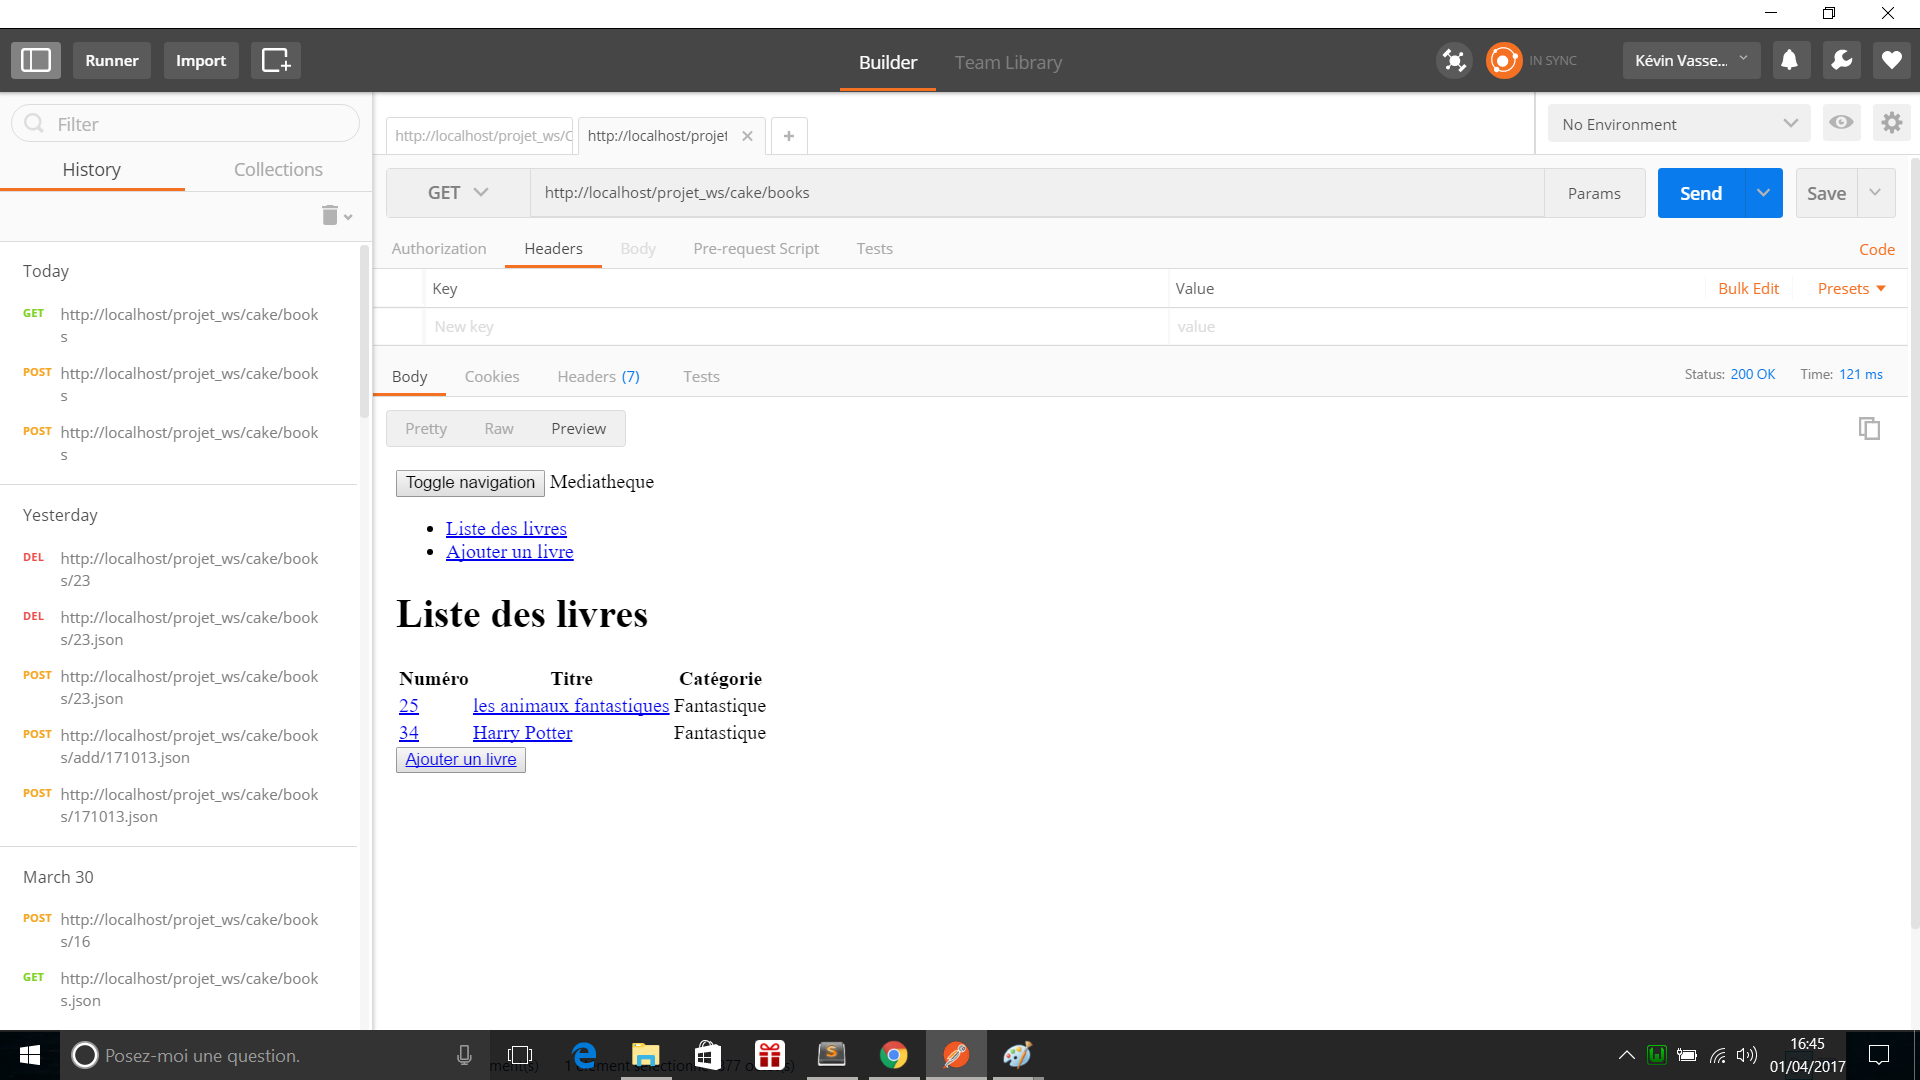
\includegraphics[scale=0.4]{resultats/q1.png} 
		\end{center} 
		\subsection{Question 2}
		\begin{center}
			\includegraphics[scale=0.4]{resultats/q2.png} 
		\end{center} 
		\subsection{Question 3}
		\begin{center}
			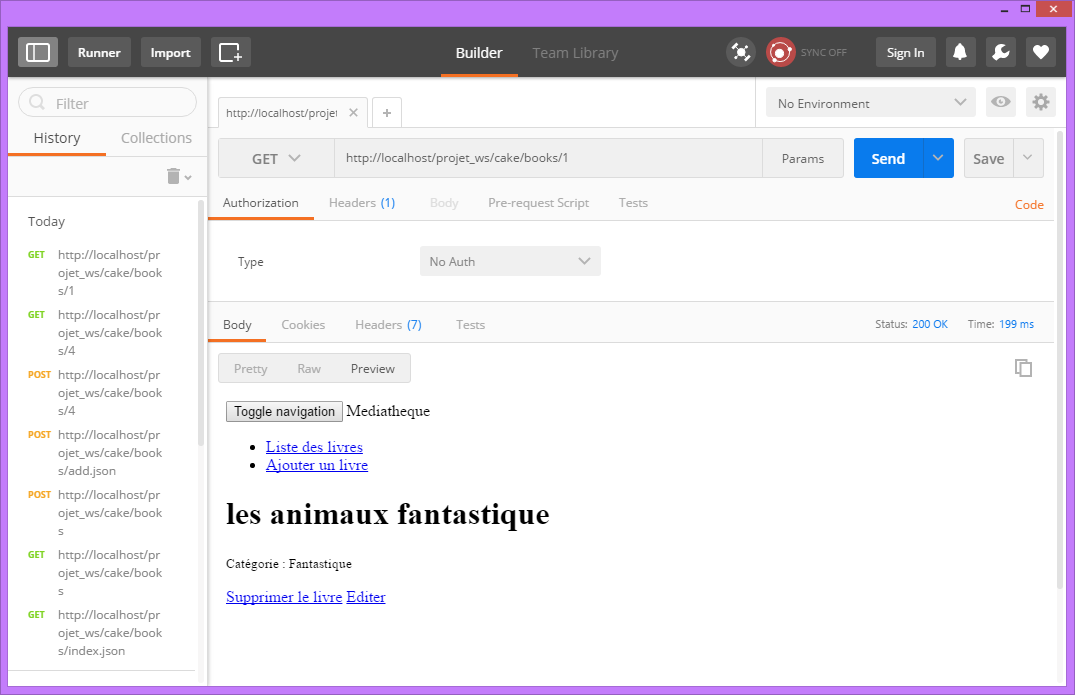
\includegraphics[scale=0.4]{resultats/q3.png} 
		\end{center} 
		\subsection{Question 4}
		\begin{center}
			\includegraphics[scale=0.4]{resultats/q4.png} 
		\end{center} 
		\subsection{Question 5}
		\begin{center}
			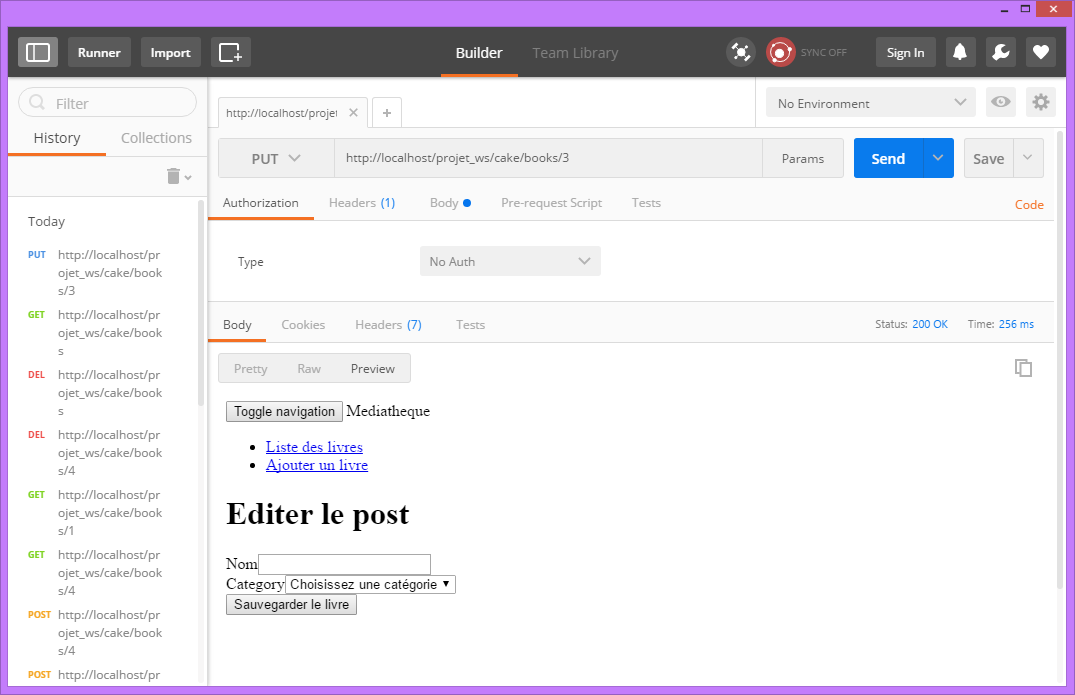
\includegraphics[scale=0.4]{resultats/q5.png} 
		\end{center} 
		\subsection{Question 6}
		\begin{center}
			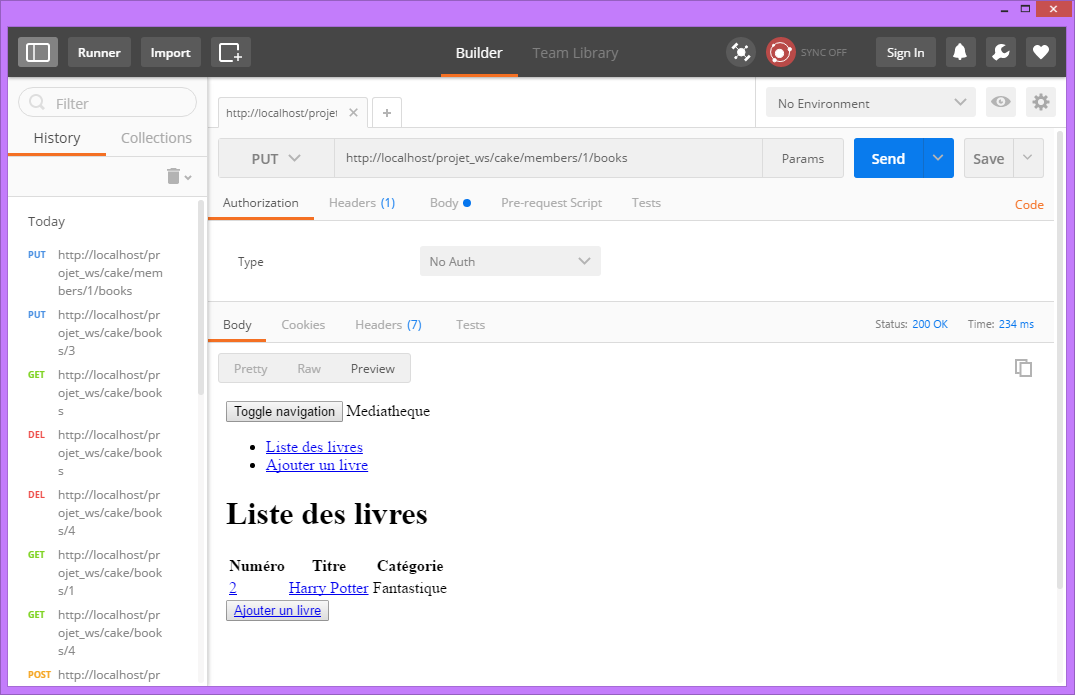
\includegraphics[scale=0.4]{resultats/q6.png} 
		\end{center} 
		
	\section{Liens}
		\href{https://github.com/kvasseur/webservices}{Github} \\
		\href{https://trello.com/b/A1vuuQZb/webservices-api-rest-mediatheque}{Trello}
	
	
	% ########## DOCUMENTATION ##########	
	\chapter{Manuel d'installation}
	
	\begin{enumerate}
		\item Si vous ne poss\'{e}dez pas l'environnement WAMP, vous pouvez la t\'{e}l\'{e}charger sur le site officiel : \href{http://www.wampserver.com/}{WAMP}\\
		Un tutoriel d'installation est disponible sur ce site: \href{http://www.cndp.fr/crdp-dijon/Installer-et-configurer-Wampserver.html}{lien}
		\item Mettre le fichier \textit{"projet\_ws"} dans le fichier \textit{"www"} (chemin : C:\textbackslash wamp\textbackslash www)
		\item Acc\'{e}der au site avec le lien: \url{http://localhost/projet_ws/cake/books}
	\end{enumerate}
	
	\begin{center}
	
\includegraphics[scale=0.1]{img/fioritures.png} 
	\end{center} 
	
	\chapter{Manuel d'utilisation}
	
	
	
	
\end{document}